% Options for packages loaded elsewhere
\PassOptionsToPackage{unicode}{hyperref}
\PassOptionsToPackage{hyphens}{url}
\PassOptionsToPackage{dvipsnames,svgnames,x11names}{xcolor}
%
\documentclass[
]{agujournal2019}

\usepackage{amsmath,amssymb}
\usepackage{iftex}
\ifPDFTeX
  \usepackage[T1]{fontenc}
  \usepackage[utf8]{inputenc}
  \usepackage{textcomp} % provide euro and other symbols
\else % if luatex or xetex
  \usepackage{unicode-math}
  \defaultfontfeatures{Scale=MatchLowercase}
  \defaultfontfeatures[\rmfamily]{Ligatures=TeX,Scale=1}
\fi
\usepackage{lmodern}
\ifPDFTeX\else  
    % xetex/luatex font selection
\fi
% Use upquote if available, for straight quotes in verbatim environments
\IfFileExists{upquote.sty}{\usepackage{upquote}}{}
\IfFileExists{microtype.sty}{% use microtype if available
  \usepackage[]{microtype}
  \UseMicrotypeSet[protrusion]{basicmath} % disable protrusion for tt fonts
}{}
\makeatletter
\@ifundefined{KOMAClassName}{% if non-KOMA class
  \IfFileExists{parskip.sty}{%
    \usepackage{parskip}
  }{% else
    \setlength{\parindent}{0pt}
    \setlength{\parskip}{6pt plus 2pt minus 1pt}}
}{% if KOMA class
  \KOMAoptions{parskip=half}}
\makeatother
\usepackage{xcolor}
\setlength{\emergencystretch}{3em} % prevent overfull lines
\setcounter{secnumdepth}{5}
% Make \paragraph and \subparagraph free-standing
\ifx\paragraph\undefined\else
  \let\oldparagraph\paragraph
  \renewcommand{\paragraph}[1]{\oldparagraph{#1}\mbox{}}
\fi
\ifx\subparagraph\undefined\else
  \let\oldsubparagraph\subparagraph
  \renewcommand{\subparagraph}[1]{\oldsubparagraph{#1}\mbox{}}
\fi


\providecommand{\tightlist}{%
  \setlength{\itemsep}{0pt}\setlength{\parskip}{0pt}}\usepackage{longtable,booktabs,array}
\usepackage{calc} % for calculating minipage widths
% Correct order of tables after \paragraph or \subparagraph
\usepackage{etoolbox}
\makeatletter
\patchcmd\longtable{\par}{\if@noskipsec\mbox{}\fi\par}{}{}
\makeatother
% Allow footnotes in longtable head/foot
\IfFileExists{footnotehyper.sty}{\usepackage{footnotehyper}}{\usepackage{footnote}}
\makesavenoteenv{longtable}
\usepackage{graphicx}
\makeatletter
\def\maxwidth{\ifdim\Gin@nat@width>\linewidth\linewidth\else\Gin@nat@width\fi}
\def\maxheight{\ifdim\Gin@nat@height>\textheight\textheight\else\Gin@nat@height\fi}
\makeatother
% Scale images if necessary, so that they will not overflow the page
% margins by default, and it is still possible to overwrite the defaults
% using explicit options in \includegraphics[width, height, ...]{}
\setkeys{Gin}{width=\maxwidth,height=\maxheight,keepaspectratio}
% Set default figure placement to htbp
\makeatletter
\def\fps@figure{htbp}
\makeatother
% definitions for citeproc citations
\NewDocumentCommand\citeproctext{}{}
\NewDocumentCommand\citeproc{mm}{%
  \begingroup\def\citeproctext{#2}\cite{#1}\endgroup}
% avoid brackets around text for \cite:
\makeatletter
 \def\@biblabel#1{}
 \def\@cite#1#2{{#1\if@tempswa , #2\fi}}
\makeatother
\newlength{\cslhangindent}
\setlength{\cslhangindent}{1.5em}
\newlength{\csllabelwidth}
\setlength{\csllabelwidth}{3em}
\newlength{\cslentryspacing}
\setlength{\cslentryspacing}{0em}
\usepackage{enumitem}
\newlist{CSLReferences}{itemize}{1}
\setlist[CSLReferences]{label={},
  leftmargin=\cslhangindent,
  itemindent=-1\cslhangindent,
  parsep=\parskip,
  itemsep=\cslentryspacing}
\usepackage{calc}
\newcommand{\CSLBlock}[1]{#1\hfill\break}
\newcommand{\CSLLeftMargin}[1]{\parbox[t]{\csllabelwidth}{#1}}
\newcommand{\CSLRightInline}[1]{\parbox[t]{\linewidth - \csllabelwidth}{#1}\break}
\newcommand{\CSLIndent}[1]{\hspace{\cslhangindent}#1}

\usepackage{url} %this package should fix any errors with URLs in refs.
\usepackage{lineno}
\usepackage[inline]{trackchanges} %for better track changes. finalnew option will compile document with changes incorporated.
\usepackage{soul}
\linenumbers
\makeatletter
\makeatother
\makeatletter
\makeatother
\makeatletter
\@ifpackageloaded{caption}{}{\usepackage{caption}}
\AtBeginDocument{%
\ifdefined\contentsname
  \renewcommand*\contentsname{Table of contents}
\else
  \newcommand\contentsname{Table of contents}
\fi
\ifdefined\listfigurename
  \renewcommand*\listfigurename{List of Figures}
\else
  \newcommand\listfigurename{List of Figures}
\fi
\ifdefined\listtablename
  \renewcommand*\listtablename{List of Tables}
\else
  \newcommand\listtablename{List of Tables}
\fi
\ifdefined\figurename
  \renewcommand*\figurename{Figure}
\else
  \newcommand\figurename{Figure}
\fi
\ifdefined\tablename
  \renewcommand*\tablename{Table}
\else
  \newcommand\tablename{Table}
\fi
}
\@ifpackageloaded{float}{}{\usepackage{float}}
\floatstyle{ruled}
\@ifundefined{c@chapter}{\newfloat{codelisting}{h}{lop}}{\newfloat{codelisting}{h}{lop}[chapter]}
\floatname{codelisting}{Listing}
\newcommand*\listoflistings{\listof{codelisting}{List of Listings}}
\makeatother
\makeatletter
\@ifpackageloaded{caption}{}{\usepackage{caption}}
\@ifpackageloaded{subcaption}{}{\usepackage{subcaption}}
\makeatother
\makeatletter
\@ifpackageloaded{sidenotes}{}{\usepackage{sidenotes}}
\@ifpackageloaded{marginnote}{}{\usepackage{marginnote}}
\makeatother
\makeatletter
\makeatother
\ifLuaTeX
  \usepackage{selnolig}  % disable illegal ligatures
\fi
\IfFileExists{bookmark.sty}{\usepackage{bookmark}}{\usepackage{hyperref}}
\IfFileExists{xurl.sty}{\usepackage{xurl}}{} % add URL line breaks if available
\urlstyle{same} % disable monospaced font for URLs
\hypersetup{
  pdftitle={La Palma Earthquakes},
  pdfauthor={Steve Purves; Rowan Cockett},
  pdfkeywords={La Palma, Earthquakes},
  colorlinks=true,
  linkcolor={blue},
  filecolor={Maroon},
  citecolor={Blue},
  urlcolor={Blue},
  pdfcreator={LaTeX via pandoc}}

\journalname{Notebooks Now!}

\draftfalse

\begin{document}
\title{La Palma Earthquakes}

\authors{Steve Purves\affil{1}, Rowan Cockett\affil{1}}
\affiliation{1}{Curvenote, }
\correspondingauthor{Steve Purves}{steve@curvenote.com}

\begin{keypoints}
\item You may specify 1 to 3 keypoints for this PDF template \item These
keypoints are complete sentences and less than or equal to 140
characters \item They are specific to this PDF template, so they will
not appear in other exports 
\end{keypoints}

\begin{abstract}
In September 2021, a significant jump in seismic activity on the island
of La Palma (Canary Islands, Spain) signaled the start of a volcanic
crisis that still continues at the time of writing. Earthquake data is
continually collected and published by the Instituto Geográphico
Nacional (IGN). We have created an accessible dataset from this and
completed preliminary data analysis which shows seismicity originating
at two distinct depths, consistent with the model of a two reservoir
system feeding the currently very active volcano.
\end{abstract}



\subsection{Introduction}\label{introduction}

La Palma is one of the west most islands in the Volcanic Archipelago of
the Canary Islands, a Spanish territory situated is the Atlantic Ocean
where at their closest point are 100km from the African coast
Figure~\ref{fig-map}. The island is one of the youngest, remains active
and is still in the island forming stage.

\begin{figure}

{\centering 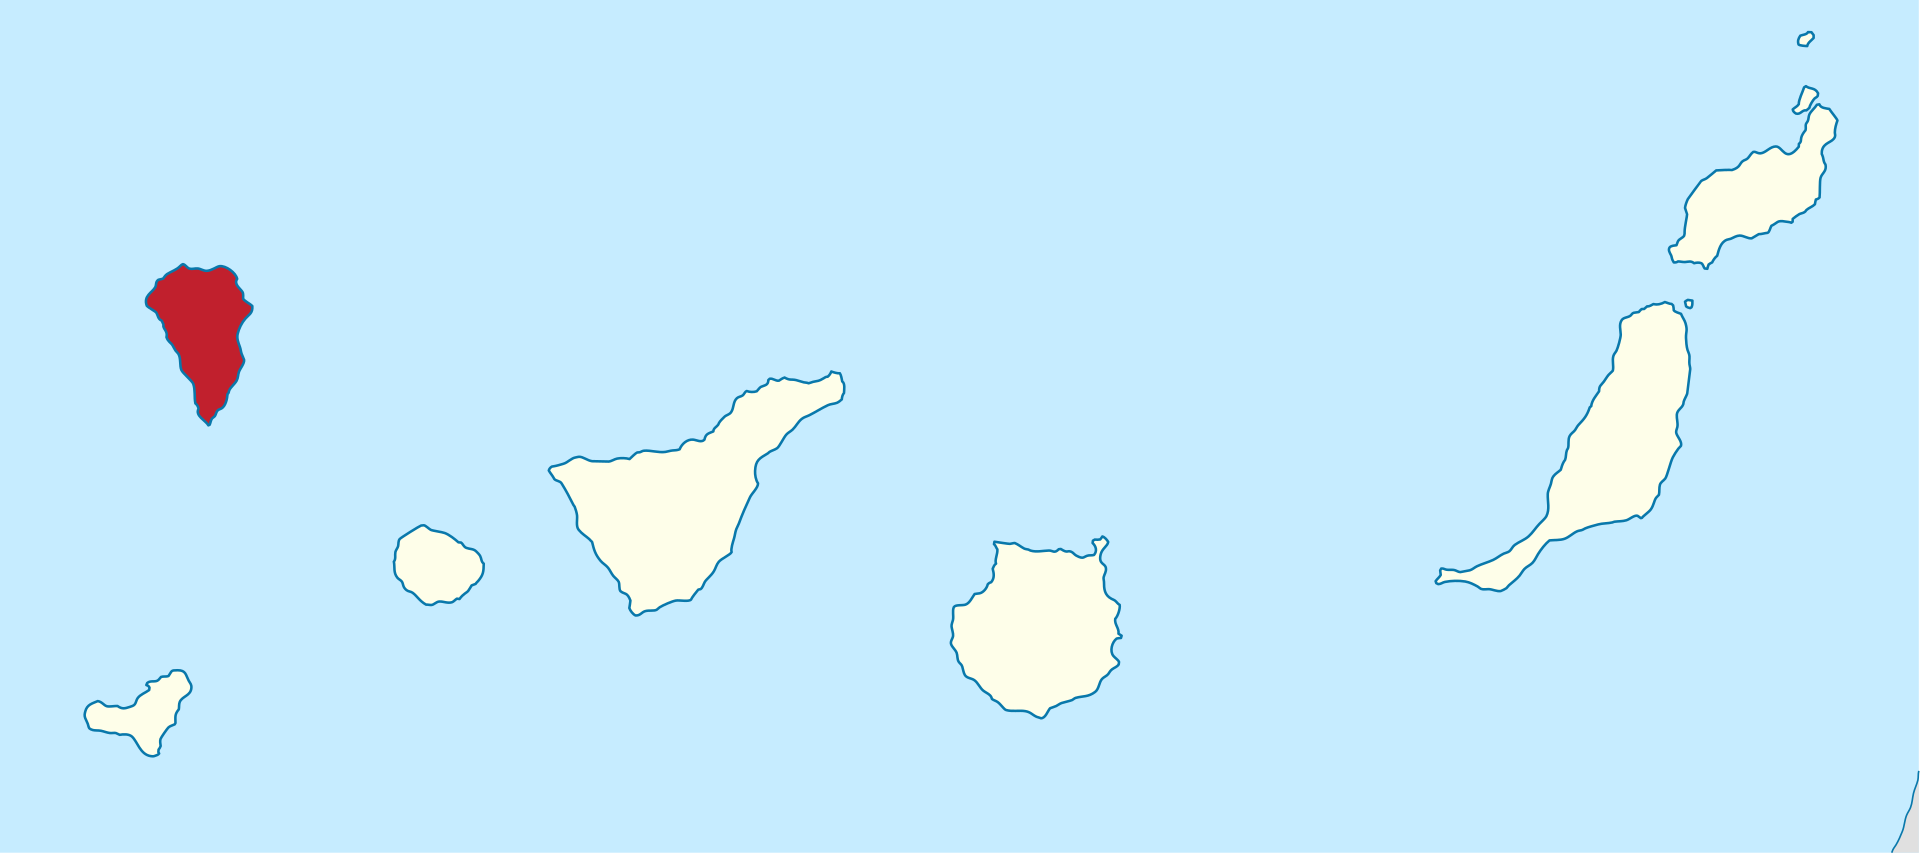
\includegraphics[width=1\textwidth,height=\textheight]{images/la-palma-map.png}

}

\caption{\label{fig-map}Map of La Palma in the Canary Islands. Image
credit
\href{https://commons.wikimedia.org/w/index.php?curid=76638603}{NordNordWest}
Source:
\href{https://Notebooks-Now.github.io/submission-quarto-lite/article.ipynb.html}{Article
Notebook}}

\end{figure}

La Palma has been constructed by various phases of volcanism, the most
recent and currently active being the \emph{Cumbre Vieja} volcano, a
north-south volcanic ridge that constitutes the southern half of the
island.

\subsubsection{Eruption History}\label{eruption-history}

A number of eruptions were recorded since the colonization of the
islands by Europeans in the late 1400s, these are summarised in
Table~\ref{tbl-history}.

\begin{longtable}[]{@{}ll@{}}
\caption{\label{tbl-history}Recent historic eruptions on La
Palma}\tabularnewline
\toprule\noalign{}
Name & Year \\
\midrule\noalign{}
\endfirsthead
\toprule\noalign{}
Name & Year \\
\midrule\noalign{}
\endhead
\bottomrule\noalign{}
\endlastfoot
Current & 2021 \\
Teneguía & 1971 \\
Nambroque & 1949 \\
El Charco & 1712 \\
Volcán San Antonio & 1677 \\
Volcán San Martin & 1646 \\
Tajuya near El Paso & 1585 \\
Montaña Quemada & 1492 \\
\end{longtable}

This equates to an eruption on average every 79 years up until the 1971
event. The probability of a future eruption can be modeled by a Poisson
distribution Equation~\ref{eq-poisson}.

\begin{equation}\phantomsection\label{eq-poisson}{
p(x)=\frac{e^{-\lambda} \lambda^{x}}{x !}
}\end{equation}

Where \(\lambda\) is the number of eruptions per year,
\(\lambda=\frac{1}{79}\) in this case. The probability of a future
eruption in the next \(t\) years can be calculated by:

\begin{equation}\phantomsection\label{eq-probability}{
p_e = 1-\mathrm{e}^{-t \lambda}
}\end{equation}

So following the 1971 eruption the probability of an eruption in the
following 50 years --- the period ending this year --- was 0.469. After
the event, the number of eruptions per year moves to
\(\lambda=\frac{1}{75}\) and the probability of a further eruption
within the next 50 years (2022-2071) rises to 0.487 and in the next 100
years, this rises again to 0.736.

\subsubsection{Magma Reservoirs}\label{magma-reservoirs}

Studies of the magma systems feeding the volcano, such as Marrero et al.
(2019) has proposed that there are two main magma reservoirs feeding the
Cumbre Vieja volcano; one in the mantle (30-40km depth) which charges
and in turn feeds a shallower crustal reservoir (10-20km depth).

\begin{figure}

{\centering 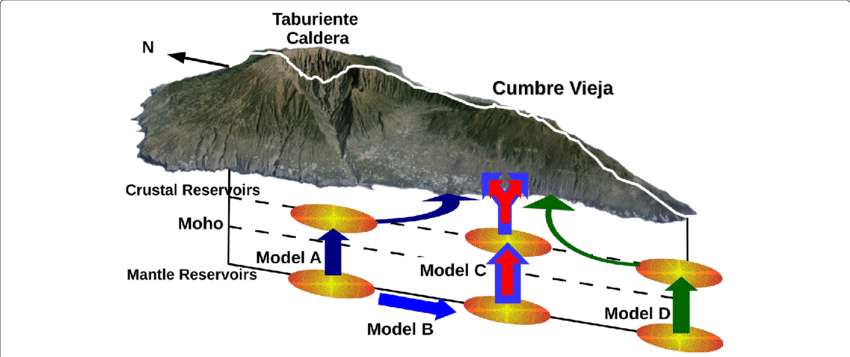
\includegraphics[width=1\textwidth,height=\textheight]{images/reservoirs.png}

}

\caption{\label{fig-reservoirs}Proposed model from Marrero et al Source:
\href{https://Notebooks-Now.github.io/submission-quarto-lite/article.ipynb.html}{Article
Notebook}}

\end{figure}

In this paper, we look at recent seismicity data to see if we can see
evidence of such a system action, see Figure~\ref{fig-reservoirs}.

\subsection{Dataset}\label{dataset}

The earthquake dataset used in our analysis was generated from the
\href{https://www.ign.es/web/resources/volcanologia/tproximos/canarias.html}{IGN
web portal} this is public data released under a permissive license.
Data recorded using the network of Seismic Monitoring Stations on the
island. A web scraping script was developed to pull data into a
machine-readable form for analysis. That code tool
\href{https://github.com/stevejpurves/ign-earthquake-data}{is available
on GitHub} along with a copy of recently updated data.

\subsection{Main Timeline Figure}\label{main-timeline-figure}

\subsection{Visualising Long term earthquake
data}\label{visualising-long-term-earthquake-data}

Data taken directly from the IGN Catalog

\begin{figure*}[H]

{\centering 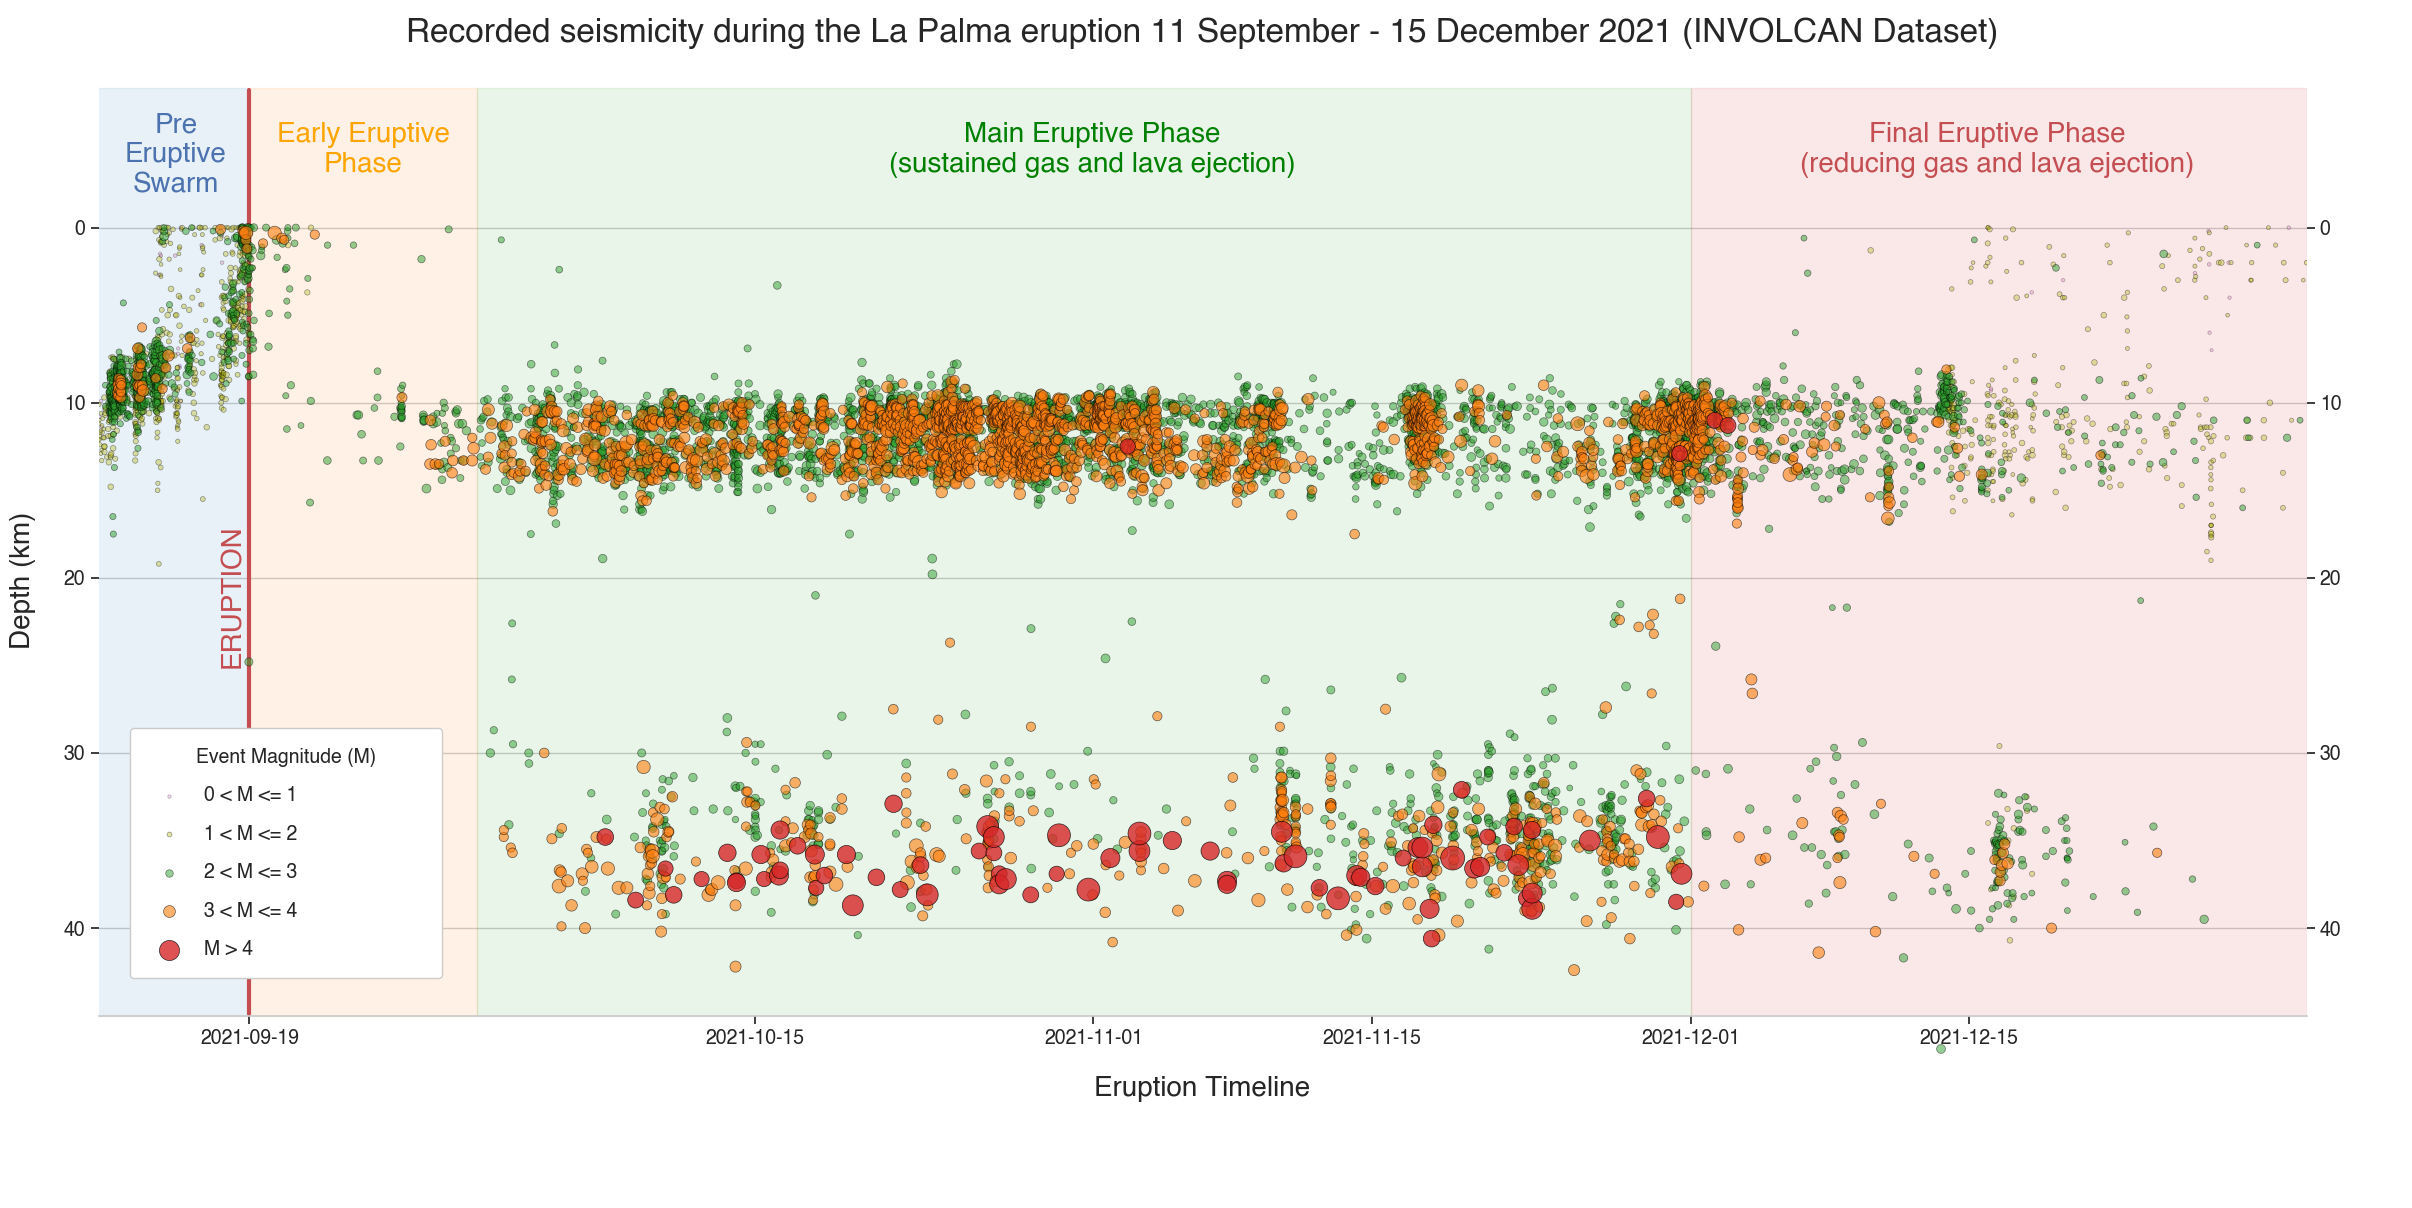
\includegraphics{article_files/figure-pdf/fig-timeline-output-1.png}

}

\caption{\label{fig-timeline}Earthquake data over time (n=5465) to
understand their distributions spatially, by depth, by magnitude and in
time. Source:
\href{https://Notebooks-Now.github.io/submission-quarto-lite/article.ipynb.html}{Article
Notebook}}

\end{figure*}

\subsection{Cumulative Distribution
Plots}\label{cumulative-distribution-plots}

\begin{figure}[H]

{\centering 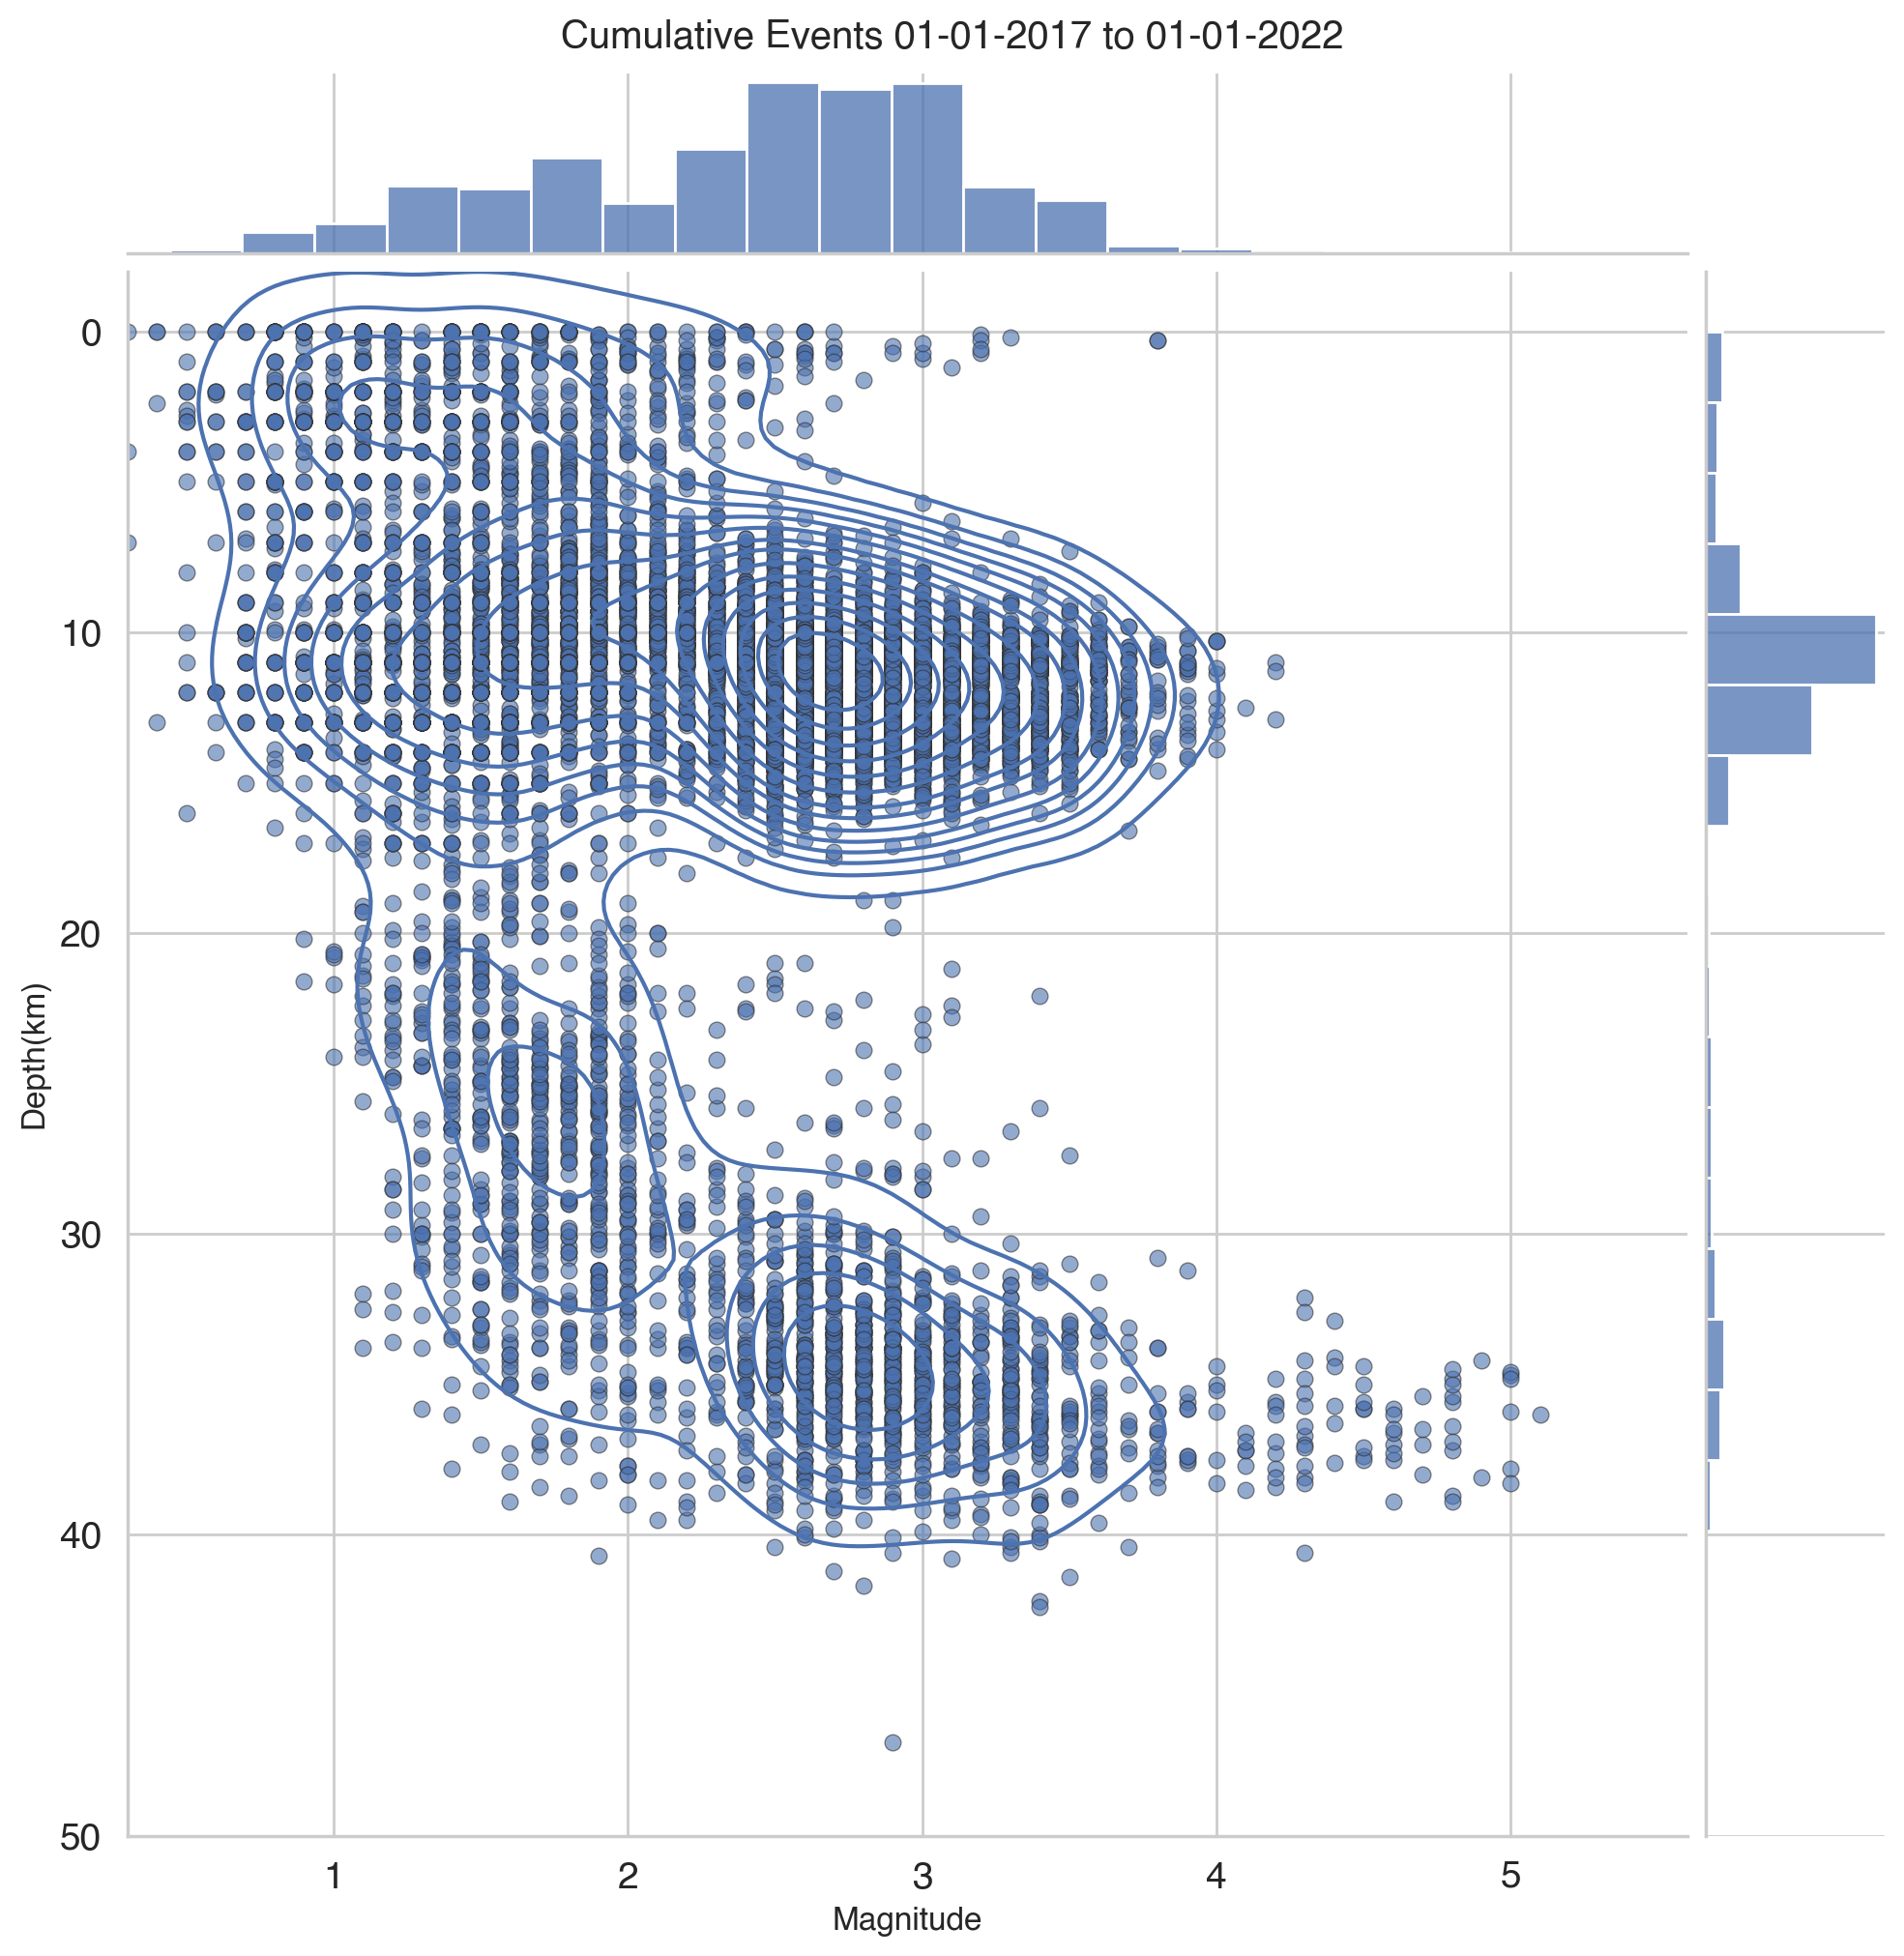
\includegraphics{article_files/figure-pdf/fig-cumulative-output-1.png}

}

\caption{\label{fig-cumulative}Cumulative earthquake data over time
(n=5465) to understand their distributions spatially, by depth and
magnitude. Source:
\href{https://Notebooks-Now.github.io/submission-quarto-lite/article.ipynb.html}{Article
Notebook}}

\end{figure}

\subsection{Results}\label{results}

The dataset was loaded into this Jupyter notebook and filtered down to
La Palma events only. This results in 5465 data points which we then
visualized to understand their distributions spatially, by depth, by
magnitude and in time.

From our analysis above, we can see 3 different systems in play.

Firstly, the shallow earthquake swarm leading up to the eruption on 19th
September, related to significant surface deformation and shallow magma
intrusion.

After the eruption, continuous shallow seismicity started at 10-15km
corresponding to magma movement in the crustal reservoir.

Subsequently, high magnitude events begin occurring at 30-40km depths
corresponding to changes in the mantle reservoir. These are also
continuous but occur with a lower frequency than in the crustal
reservoir.

\subsection{Conclusions}\label{conclusions}

From the analysis of the earthquake data collected and published by IGN
for the period of 11 September through to 9 November 2021. Visualization
of the earthquake events at different depths appears to confirm the
presence of both mantle and crustal reservoirs as proposed by Marrero et
al. (2019).

\subsection{Availability}\label{availability}

A web scraping script was developed to pull data into a machine-readable
form for analysis. That code tool
\href{https://github.com/stevejpurves/ign-earthquake-data}{is available
on GitHub} along with a copy of recently updated data.

\subsection*{References}\label{references}
\addcontentsline{toc}{subsection}{References}

\phantomsection\label{refs}
\setlength{\cslentryspacing}{0em}
\begin{CSLReferences}
\bibitem[\citeproctext]{ref-marrero2019}
Marrero, J., García, A., Berrocoso, M., Llinares, Á., Rodríguez-Losada,
A., \& Ortiz, R. (2019). Strategies for the development of volcanic
hazard maps in monogenetic volcanic fields: The example of {La} {Palma}
({Canary} {Islands}). \emph{Journal of Applied Volcanology}, \emph{8}.
\url{https://doi.org/10.1186/s13617-019-0085-5}

\end{CSLReferences}



\end{document}
